\documentclass[aspectratio=169,
				xcolor=table]{beamer}

% Load general definitions
\usepackage[utf8]{inputenc}
%\usepackage[T1]{fontenc}
\usepackage[brazil]{babel}
\usepackage{amsmath}
\usepackage{amsfonts}
\usepackage{amssymb}
\usepackage{graphicx}
\usepackage{verbatim}
\usepackage{cancel}
\usepackage{askmaps}
\usepackage{tabularx}
\usepackage[table]{xcolor}
%\usepackage{tikz}
\usepackage{multirow}
\usepackage{mathtools}
\usepackage{color, colortbl}
\usepackage{etoolbox}
\usepackage{pbox}
\usepackage{changepage}
\usepackage{xpatch}
\usepackage{array}
\usepackage{marvosym}
\usepackage{tabu}
\usepackage{multicol}
\usepackage{listings}
\usepackage{underscore}
\usepackage{filecontents}
\usepackage[]{algorithm2e}
\usepackage{ragged2e}

\newcolumntype{P}[1]{>{\centering\arraybackslash}m{#1}}
\definecolor{Gray}{gray}{0.75}
\definecolor{Gray2}{gray}{0.85}

\definecolor{lightBlue}{HTML}{DAE8FC}
\definecolor{Blue}{RGB}{51, 51, 204}

%\useinnertheme[lily]{rounded}
\usetheme{UniEvangelica}
%\usetheme{Copenhagen}
%\usetheme{Berlin}
%\usecolortheme{dolphin}
\tolerance=1
\emergencystretch=\maxdimen
\hyphenpenalty=10000
\hbadness=10000

\setbeamertemplate{navigation symbols}{}%remove navigation symbols


\let\olditem=\item% 
\renewcommand{\item}{\olditem \justifying}%
\def\center{\trivlist \centering\item\relax}
\def\endcenter{\endtrivlist}

\setbeamertemplate{itemize/enumerate body begin}{\large}
\setbeamertemplate{itemize/enumerate subbody begin}{\large}

\setbeamertemplate{itemize item}{\raisebox{0.1ex}{$\blacktriangleright$}\hskip0.1em}
\setbeamertemplate{itemize subitem}{\raisebox{0.1ex}{$\blacktriangleright$}\hskip0.1em}

\newcommand{\greenarrow}{\textcolor{green}{\rotatebox[origin=c]{180}{\MVArrowDown}}}

\newcommand{\redarrow}{\textcolor{red}{\MVArrowDown}}

%\newcommand{\ftable}{
%	\begin{table}
%		\large
%		\centering
%		\rowcolors{1}{\ifnumless{\rownum}{2}{Blue}{lightBlue}}{}
%}

\newenvironment{eftable}{
	\begin{table}
		\large
		\centering
		\rowcolors{1}{}{Blue}
		\rowcolors{1}{\ifnumless{\rownum}{2}{Blue}{lightBlue}}{}
	}
	{
	\end{table}
}


%\setbeamertemplate{frametitle}
%{
%	%\vspace*{-2em}	
%	\insertframetitle
%
%	 %\textcolor{white}{\LARGE \insertframetitle}
%
%}

% Specific definitions
\institute[]{\uppercase{Engenharia de Software}}
\title[]{Sistemas Operacionais}
\subtitle[]{\uppercase{Conceitos Básicos}}
\author[]{Prof. M.e Alexandre Tannus}
\date{Anápolis - 2021.1}

%\AtBeginSection{\frame{\tableofcontents[currentsection]}}

\begin{document}
	\begin{frame}
		\titlepage
		
	\end{frame}

	\begin{frame}
		\tableofcontents
	\end{frame}	
	
	\section{Introdução}
	
	\begin{frame}
		\frametitle{Questionamentos}
		\begin{itemize}
			\item O que é um sistema operacional?
			\vspace{1em}
			\item Quais são as suas funções?
			\vspace{1em}
			\item Qual é a sua estrutura fundamental?
		\end{itemize}
	\end{frame}	
	
	\begin{frame}
		\frametitle{Relembrando...}
		\begin{itemize}
			\item Sistema computacional
			\begin{itemize}
				\item CPU
				\item Memória
				\item Dispositivos de E/S
			\end{itemize}
		\end{itemize}	
		\vspace{1em}
		\begin{block}{Problema}			
			\alert{Complexidade de entendimento detalhado de cada elemento }
						

		\end{block}			
	\end{frame}
	
	\begin{frame}{Objetivos de um Sistema Operacional}
		\begin{itemize}
			\item Gerenciamento de Recursos
			\item Interface entre programador e os recursos do hardware
		\end{itemize}
	\end{frame}
	
	\begin{frame}
		\frametitle{Conceitos}
		\begin{itemize}
			\item \textit{Hardware}
			\begin{itemize}
				\item Parte física do sistema computacional
			\end{itemize}
			\vspace{1em}
			\item \textit{Software}
			\begin{itemize}
				\item Programas 
			\end{itemize}
			\vspace{1em}
			\item \textit{Firmware}
			\begin{itemize}
				\item Conjunto de instruções operacionais programadas diretamente no \textit{hardware}
			\end{itemize}
			\vspace{1em}
		\end{itemize}
	\end{frame}
	
	\begin{frame}{Sistema Operacional}
		\begin{itemize}
			\item ``Os computadores tem um dispositivo de software cujo trabalho é fornecer aos programas do usuário um modelo de computador melhor, mais simples e mais limpo e lidar com o gerenciamento de todos os recursos'' - Tanenbaum 			
		\end{itemize}
			\begin{figure}[hbtp]
	\centering
	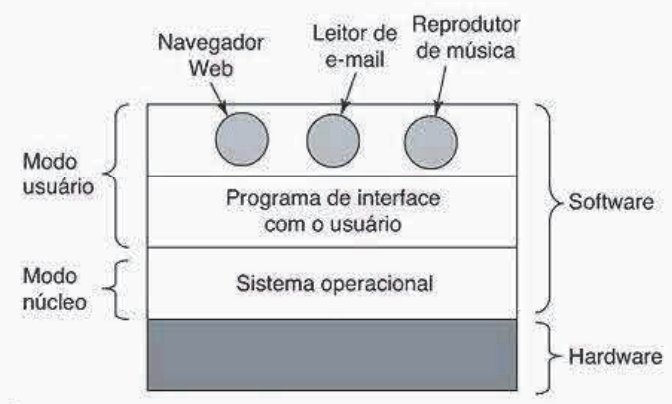
\includegraphics[height=.55\textheight, keepaspectratio]{../figs/cap01/so}
	\end{figure}
	\end{frame}
	
	\section{Histórico}
	\begin{frame}{${1}^{a}$ Geração de Computadores}
		\begin{itemize}
			\item Construídos com válvulas
			\vspace{1em}
			\item Programação em código de máquina
			\vspace{1em}
			\item Ausência de sistemas operacionais
		\end{itemize}
	\end{frame}
	
	\begin{frame}{${2}^{a}$ Geração de Computadores}
		\begin{itemize}
			\item Introdução dos transistores
			\vspace{1em}
			\item Computadores de grande porte (\textit{mainframes})
			\vspace{1em}
			\item Sistema de processamento em lote (\textit{batch})
		\end{itemize}
	\end{frame}
	
	\begin{frame}{Processamento \textit{batch}}
	\begin{figure}[hbtp]
	\centering
	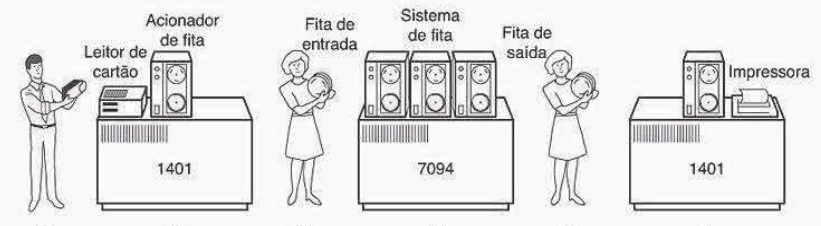
\includegraphics[width=.85\textwidth, keepaspectratio]{../figs/cap01/batch.png}
	\end{figure}
	
	\end{frame}
	
	\begin{frame}{Processamento \textit{batch}}
	\begin{figure}[hbtp]
	\centering
	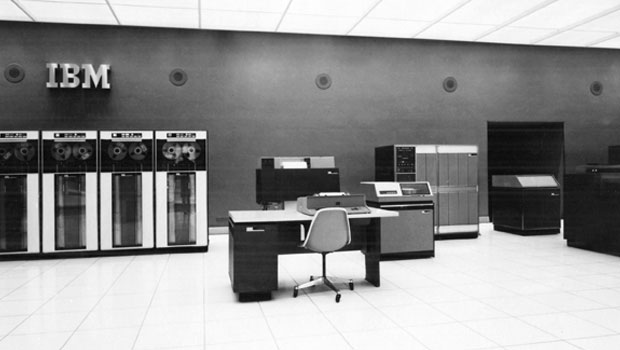
\includegraphics[height=.75\textheight, keepaspectratio]{../figs/cap01/ibmroom}
	\end{figure}
	\end{frame}
	
	\begin{frame}{${3}^{a}$ Geração de Computadores}
		\begin{itemize}
			\item Circuitos integrados - Integração em larga escala
			\vspace{1em}
			\item Computadores de propósito geral
			\vspace{1em}
			\item Sistema operacional IBM OS/360
			\vspace{1em}
			\item \alert{Multiprogramação}
			\vspace{1em}
			\item \alert{\textit{Timesharing}}
		\end{itemize}
	\end{frame}
	
	\begin{frame}{Multiprogramação}
		\begin{itemize}
			\item Possibilidade de execução de várias tarefas simultaneamente
			\item Processos \textit{CPU-bound}
			\begin{itemize}
				\item Demandam alta utilização da CPU
				\item Exemplo: cálculos matemáticos
			\end{itemize}
			\item Processos \textit{IO-bound}
			\begin{itemize}
				\item Alto fluxo de entrada e saída de dados
				\item Exemplo: digitação
			\end{itemize}
		\end{itemize}
	\end{frame}
	
	\begin{frame}{Timesharing}
		\begin{itemize}
			\item Tempo compartilhado
			\begin{itemize}
				\item Alocação da CPU para tarefas que necessitam dela
			\end{itemize}
			\vspace{1em}
			\item MULTICS (\textit{Multiplexed Information and Computing Service})
			\begin{itemize}
				\item Desenvolvido por MIT, Bell Labs e General Electric
				\item Suporte para centenas de usuários simultaneamente
			\end{itemize}
		\end{itemize}
	\end{frame}

	\begin{frame}{${3}^{a}$ Geração de Computadores}
		\begin{itemize}
			\item Crescimento dos minicoputadores
			\vspace{1em}
			\item Desenvolvimento do UNIX iniciado por Ken Thompson
			\vspace{1em}
			\item Desenvolvimento do padrão POSIX
		\end{itemize}
	\end{frame}
	
\begin{frame}{${4}^{a}$ Geração de Computadores}
		\begin{itemize}
			\item Circuitos integrados VLSI
			\vspace{1em}
			\item Introdução dos microcomputadores
			\vspace{1em}
			\item Sistema operacional CP/M (\textit{Control Program for Microcomputers}) - 1974
			\vspace{1em}
			\item \textit{Disk Operating System} - DOS - 1980
		\end{itemize}
	\end{frame}	
	
	\begin{frame}{${4}^{a}$ Geração de Computadores}
		\begin{itemize}
			\item Popularização das interfaces gráficas
			\begin{itemize}
				\item Apple Macintosh
				\item Microsoft Windows
				\item X11
				\item Gnome
				\item KDE
			\end{itemize}
			\vspace{1em}
			\item Sistemas operacionais de rede
			\vspace{1em}
			\item Sistemas operacionais distribuídos
		\end{itemize}
	\end{frame}

	\section{Conceitos Fundamentais}
	
	\begin{frame}{Tipos de Sistemas Operacionais}
	\begin{itemize}
		\item Computadores de grande porte			
		\vspace{0.45em}
		\item Servidores					
		\vspace{0.45em}
		\item Multiprocessadores			
		\vspace{0.45em}
		\item Computadores pessoais
		\vspace{0.45em}		
		\item Computadores portáteis
		
	\end{itemize}
	\end{frame}

	\begin{frame}{Tipos de Sistemas Operacionais}
	\begin{itemize}
		\item Embarcados
		\vspace{0.45em}
		\item Nós sensores
		\vspace{0.45em}
		\item Tempo Real
		
	\end{itemize}
	\end{frame}	
	
	\begin{frame}{Classificação dos Sistemas Operacionais}
		\begin{itemize}
			\item Sistemas Monoprogramáveis
			\vspace{1em}
			\item Sistemas Multiprogramáveis
			\begin{itemize}
				\item \textit{Batch}
				\item Tempo compartilhado
				\item Tempo real
			\end{itemize}
			\vspace{1em}
			\item Sistemas Multiprocessadores
			\begin{itemize}
				\item Fortemente acoplados
				\item Fracamente acoplados
			\end{itemize}
		\end{itemize}
	\end{frame}
	
	\begin{frame}{Sistemas Monoprogramáveis}
		\begin{columns}
			\begin{column}{0.5\textwidth}			
				\begin{itemize}
					\item Também conhecidos como sistemas monotarefas
					\vspace{1em}
					\item Todos os recursos do sistema ficam dedicados exclusivamente a uma única tarefa
					\vspace{1em}
					\item Preocupação reduzida com problemas relacionados a compartilhamento de recursos
					\vspace{1em}
					\item Implementação simples
				\end{itemize}
			\end{column}
			\begin{column}{0.5\textwidth}
			\begin{figure}[hbtp]
				\centering
				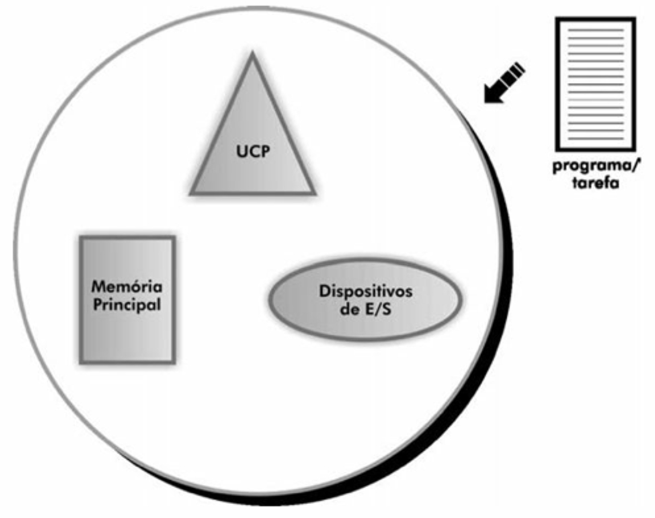
\includegraphics[width=.85\textwidth, keepaspectratio]{../figs/cap01/monotarefa.png}
			\end{figure}
			\end{column}
		\end{columns}
	\end{frame}
	
	\begin{frame}{Sistemas multiprogramáveis}
		\begin{columns}
			\begin{column}{0.5\textwidth}
				\begin{itemize}
					\item Também conhecidos como sistemas multitarefas
					\vspace{0.8em}
					\item Recursos compartilhados entre diversos usuários e aplicações
					\vspace{0.8em}
					\item Sistema operacional controla o acesso concorrente aos recursos
					\vspace{0.8em}
					\item Redução de custos e tempo médio de execução das aplicações
					\vspace{0.8em}
					\item Implementação mais complexa que a dos sistemas monotarefa
				\end{itemize}
			\end{column}
			\begin{column}{0.5\textwidth}			
				\begin{figure}[hbtp]
					\centering
					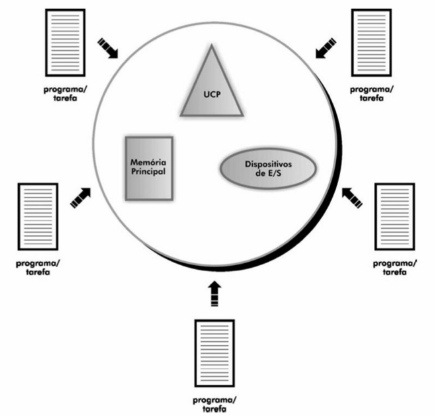
\includegraphics[width=.85\textwidth, keepaspectratio]{../figs/cap01/multitarefa.png}
				\end{figure}
			\end{column}
		\end{columns}
	\end{frame}
	
	\begin{frame}{Sistemas com Múltiplos Processadores}
		\begin{itemize}
			\item Duas ou mais CPUs interligadas
			\vspace{1em}
			\item Possibilidade de execução simultânea de aplicações ou divisão da aplicação em subpartes 
			\vspace{1em}
			\item Conceitos aplicáveis
			\begin{itemize}
				\item Escalabilidade
				\item Disponibilidade
				\item Balanceamento de carga
			\end{itemize}
			\vspace{1em}
			\item Classificação
			\begin{itemize}
				\item Fortemente acoplados
				\item Fracamente acoplados
			\end{itemize}
		\end{itemize}
	\end{frame}

	\begin{frame}{Sistemas fortemente acoplados}	
		\begin{figure}[hbtp]
			\centering
			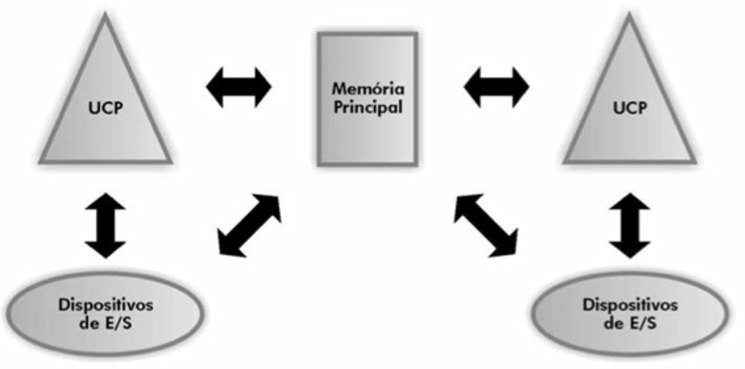
\includegraphics[width=.85\textwidth, keepaspectratio]{../figs/cap01/fortementeAcoplado.png}
		\end{figure}
	\end{frame}
	
	\begin{frame}{Sistemas fortemente acoplados}
		\begin{itemize}
			\item Compartilhamento de uma memória física única (\textit{shared memory})
			\vspace{1em}
			\item Dispositivos de E/S gerenciados por apenas um sistema operacional
			\vspace{1em}
			\item Tipos
			\begin{itemize}
				\item \textit{Symmetric Multiprocessors} - SMP
				\item \textit{Non-Uniform Memory Access} - NUMA
			\end{itemize}
		\end{itemize}
	\end{frame}
	
	\begin{frame}{Sistemas fortemente acoplados}	
		\begin{figure}[hbtp]
			\centering
			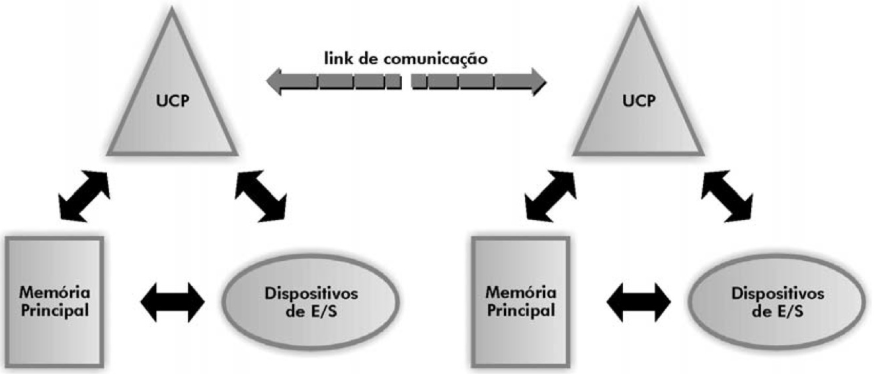
\includegraphics[width=.85\textwidth, keepaspectratio]{../figs/cap01/fracamenteAcoplado.png}
		\end{figure}
	\end{frame}
	
	\begin{frame}{Sistemas fracamente acoplados}
		\begin{itemize}
			\item Dois ou mais sistemas computacionais conectados através de linhas de comunicação
			\item Funcionamento independente de cada sistema
			\item Sistemas distribuídos
			\begin{itemize}
				\item Sistemas operacionais de rede
				\item \textit{Clusters}
			\end{itemize}
		\end{itemize}
	\end{frame}

		
	\begin{frame}
		\frametitle{Bibliografia}
		\begin{itemize}
			\item SILBERSCHATZ, A.; GALVIN, P. B.; GAGNE, G.. \textbf{Fundamentos de sistmas operacionais: princípios básicos}. Rio de Janeiro: LTC – Livros Técnicos e Científicos, 2013.


			\item ENGLANDER, Irv. \textit{A Arquitetura de Hardware Computacional, Software de Sistema e Comunicação em Rede.} 4.ed Rio de Janeiro, LTC, 2011

		\end{itemize}
	\end{frame}
	
	\begin{frame}{}
		
	\end{frame}
	
\end{document}
